\begin{figure}
    \centering
    
    % First row - Cascade profiles
    \begin{subfigure}[b]{0.3\textwidth}
        \centering
        \begin{tikzpicture}
            \begin{axis}[
                width=\textwidth,
                % xlabel={Time (s)},
                % ylabel={Bandwidth (Kbit/s)},
                ymin=0, ymax=1300, ytick distance=200,
                ymajorgrids=true,
                grid style=dashed,
                tick label style={font=\footnotesize},
                label style={font=\footnotesize},
            ]
            \addplot[red, const plot, thick, solid, mark=*] coordinates {
                (0,1200) (30,1200) (30,800) (60,800) (60,400) (90,400)
                (90,800) (120,800) (120,1200) (150,1200)
            };
            \end{axis}
        \end{tikzpicture}
        \caption{\footnotesize CASCADE}
    \end{subfigure}
    \begin{subfigure}[b]{0.3\textwidth}
        \centering
        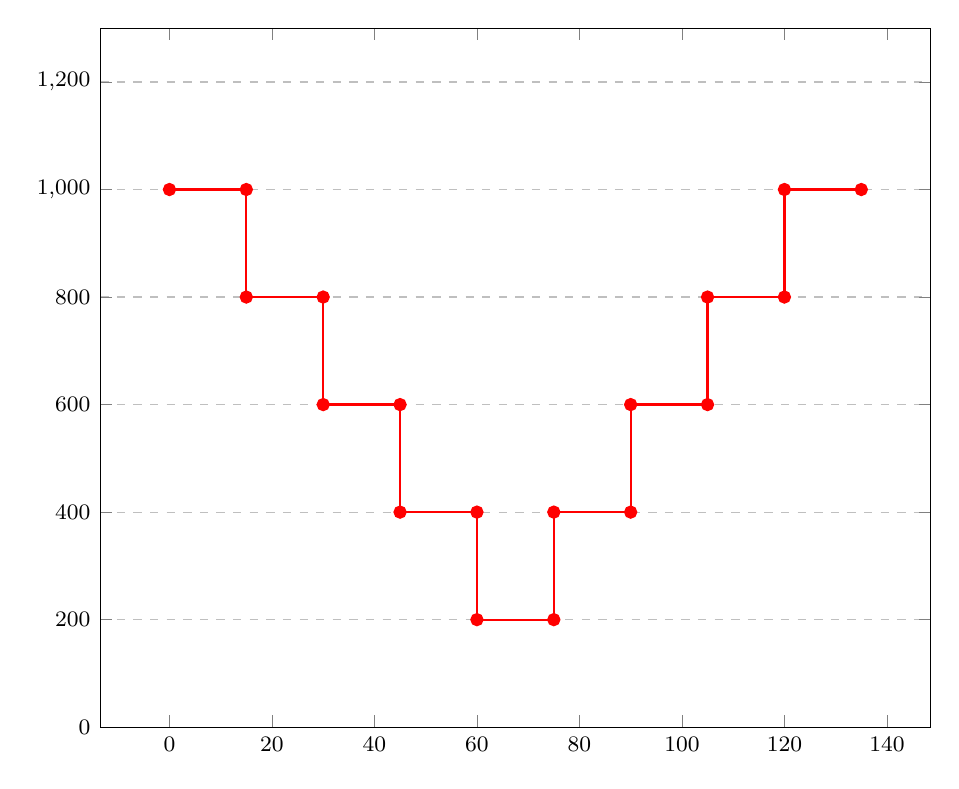
\begin{tikzpicture}
            \begin{axis}[
                width=\textwidth,
                % xlabel={Time (s)},
                % ylabel={Bandwidth (Kbit/s)},
                ymin=0, ymax=1300, ytick distance=200,
                ymajorgrids=true,
                grid style=dashed,
                tick label style={font=\footnotesize},
                label style={font=\footnotesize},
            ]
            \addplot[red, const plot, thick, solid, mark=*] coordinates {
                (0,1000) (15,1000) (15,800) (30,800) (30,600) (45,600) (45,400) (60,400)
                (60,200) (75,200) (75,400) (90,400) (90,600) (105,600) (105,800) (120,800)
                (120,1000) (135,1000)
            };
            \end{axis}
        \end{tikzpicture}
        \caption{\footnotesize INTRA\_CASCADE}
    \end{subfigure} 

    \vspace{1em}
    
    % Second row - Other profiles
    \begin{subfigure}[b]{0.3\textwidth}
        \centering
        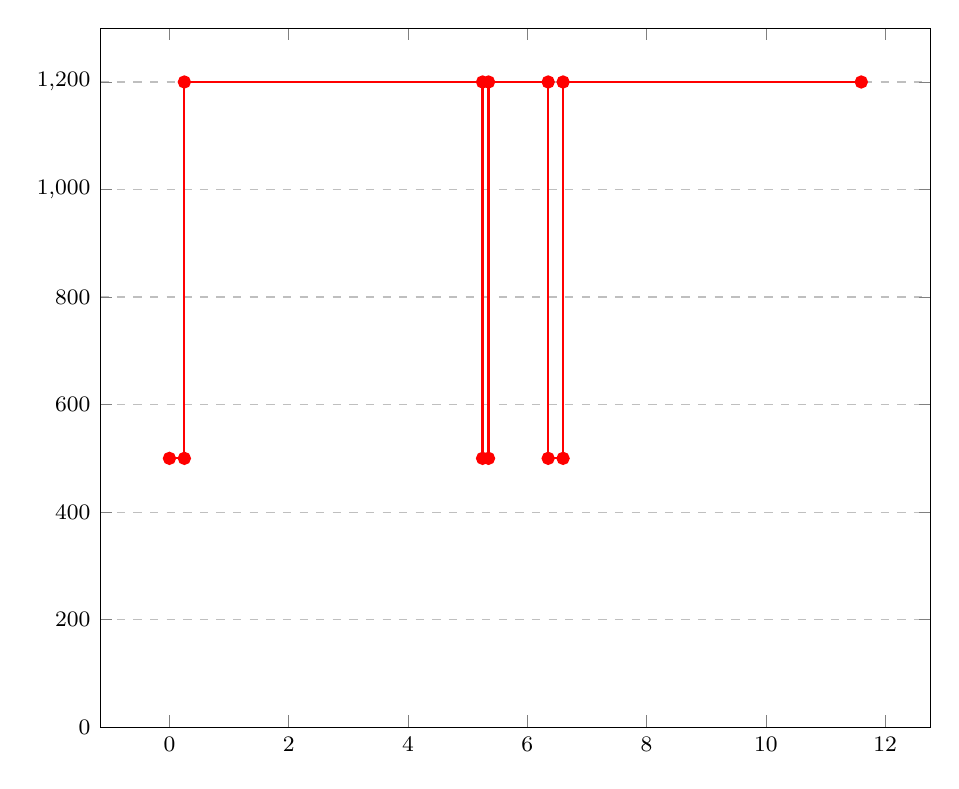
\begin{tikzpicture}
            \begin{axis}[
                width=\textwidth,
                % xlabel={Time (s)},
                % ylabel={Bandwidth (Kbit/s)},
                ymin=0, ymax=1300, ytick distance=200,
                ymajorgrids=true,
                grid style=dashed,
                tick label style={font=\footnotesize},
                label style={font=\footnotesize},
            ]
            \addplot[red, const plot, thick, solid, mark=*] coordinates {
                (0,500) (0.25,500) (0.25,1200) (5.25,1200) (5.25,500) (5.35,500)
                (5.35,1200) (6.35,1200) (6.35,500) (6.6,500) (6.6,1200) (11.6,1200)
            };
            \end{axis}
        \end{tikzpicture}
        \caption{\footnotesize FAST\_JITTERS}
    \end{subfigure}
    \begin{subfigure}[b]{0.3\textwidth}
        \centering
        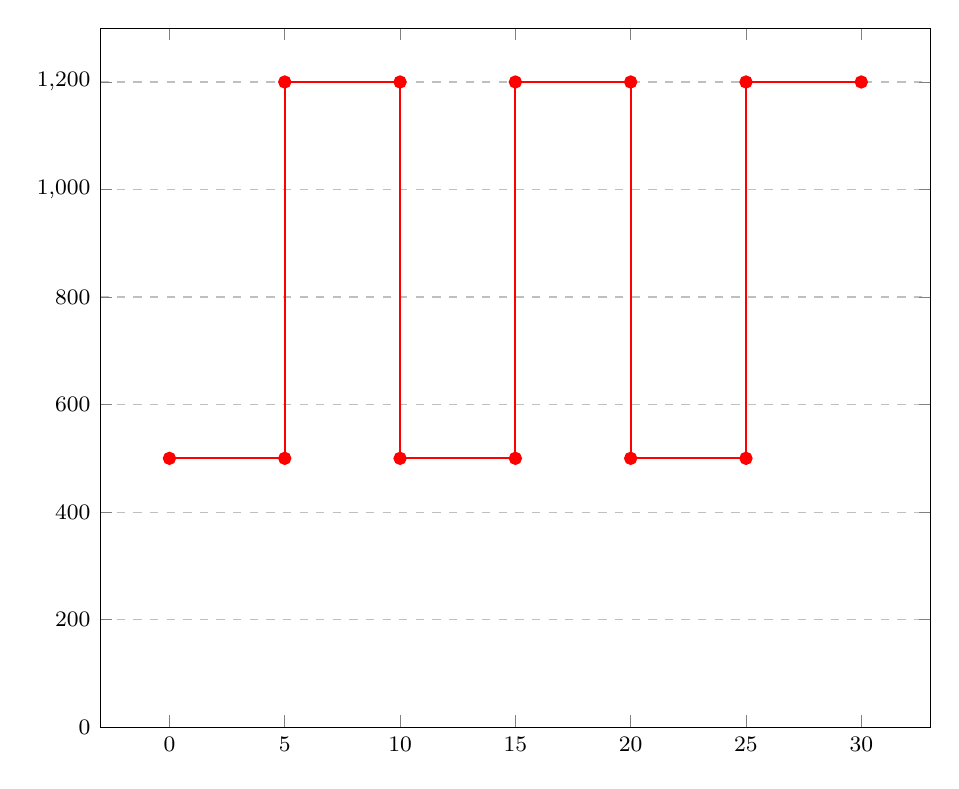
\begin{tikzpicture}
            \begin{axis}[
                width=\textwidth,
                % xlabel={Time (s)},
                % ylabel={Bandwidth (Kbit/s)},
                ymin=0, ymax=1300, ytick distance=200,
                ymajorgrids=true,
                grid style=dashed,
                tick label style={font=\footnotesize},
                label style={font=\footnotesize},
            ]
            \addplot[red, const plot, thick, solid, mark=*] coordinates {
                (0,500) (5,500) (5,1200) (10,1200) (10,500) (15,500) (15,1200) (20,1200)
                (20,500) (25,500) (25,1200) (30,1200)
            };
            \end{axis}
        \end{tikzpicture}
        \caption{\footnotesize SLOW\_JITTERS}
    \end{subfigure}
    \begin{subfigure}[b]{0.3\textwidth}
        \centering
        \begin{tikzpicture}
            \begin{axis}[
                width=\textwidth,
                % xlabel={Time (s)},
                % ylabel={Bandwidth (Kbit/s)},
                ymin=0, ymax=1300, ytick distance=200,
                ymajorgrids=true,
                grid style=dashed,
                tick label style={font=\footnotesize},
                label style={font=\footnotesize},
            ]
            \addplot[red, const plot, thick, solid, mark=*] coordinates {
                (0,1200) (10,1200) (10,300) (20,300) (20,800) (30,800)
            };
            \end{axis}
        \end{tikzpicture}
        \caption{\footnotesize SPIKE}
    \end{subfigure}

    \vspace{1em}

    \caption{Bandwidth profiles - Bandwidth (Kbit/s) vs. time (s)}
    \label{fig:bandwidth_profiles}
\end{figure}